\chapter{Свойства нано- и микромасштабных частиц, поступающих в окружающую среду при открытой разработке железорудных месторождений} \label{chapt2}

Проведено исследование свойств нано- и микромасштабных пылевых частиц, образующихся при массовых взрывах на железорудном карьере Лебединского горно-обогатительного комбината, в широком диапазоне размеров от 60 нм до 200 мкм. В ходе исследований получены данные о морфологии частиц, их магнитных свойствах, минералогическом и гранулометрическом составах. Обнаруженные минералы — кварц, магнетит и слюда. Основная часть пыли состоит из частиц разнообразной морфологии железистого кварцита, в массиве которого и производился взрыв.

\section{Введение} \label{sect2_1}

В настоящее время существенное внимание уделяется изучению нано- и микромасштабных объектов в природных и техногенных системах \cite{bib09,bib18}. Нано- и микромасштабные частицы обнаруживаются в земной коре, в тропосфере, стратосфере, ионосфере и магнитосфере Земли \cite{bib02,bib03,bib04,bib05,bib08,bib12,bib14,bib19} и играют значительную роль в явлениях, определяющих образование пылевых облаков и изменение химического состава вещества в окружающей среде. Атмосферные нано- и микромасштабные частицы и образуемые ими более крупные частицы существенным образом влияют на климатические изменения, на прозрачность и электрофизические свойства атмосферы, на перенос загрязнителей окружающей среды и биологических веществ. Наномасштабные частицы и аэрозоли участвуют в химических процессах в оболочках Земли и влияют на состояние биоты экосистем и здоровье человека. 

В науках о Земле нано- и микроразмерные компоненты выступают в качестве основных элементов ее структуры, и поэтому исследования нано- и микроразмерных объектов могут привести к расширению наших представлений о фундаментальных процессах геологии \cite{bib09}. Особый интерес с точки зрения геологии рудных месторождений представляет исследование нано- и микромасштабных пылевых частиц, образующихся при разработке полезных ископаемых и, в частности, при взрывах.

В геологических процессах важную роль играют взрывы при извержениях вулканов. Так, например, твердые продукты извержения образуются при мощных газовых взрывах. Считают, что взрывные процессы, связанные с падением крупных метеоритов на Землю (1–1.5 млрд. лет назад), повлияли на формирование минералов высокобарических фаз кремнезема и других соединений, шоковые (или планарные) структуры минералов, импактиты (ударные брекчии, состоящие из стекла, цементирующего обломки пород и минералов), раздробленные и брекчированные породы и т.д. 

Взрывы используются и для дробления рудных тел. Так, например, данные, полученные в Мурманской области в экспериментах "Днепр–1" и "Днепр–2", подтвердили расчетную эффективность использования ядерных взрывов для дробления рудных тел. 

Существенно менее мощные массовые взрывы на карьерах горнообогатительных предприятий являются одним из источников мгновенного выделения нано- и микромасштабной пыли в атмосферу – из всех источников пылеобразования при эксплуатации карьеров 60–80\% общего количества пыли приходится именно на долю массовых взрывов \cite{bib01,bib01} Значительные объемы горного производства открытым способом определяют высокую значимость проблемы воздействия массовых промышленных взрывов на окружающую среду.

Темпы роста добычи полезных ископаемых на каждого жителя Земли, составляющие около 10\% в год, существенно опережают темпы увеличения её народонаселения \cite{bib09}. Рост добычи полезных ископаемых приводит к увеличению массы одновременно взрываемых взрывчатых веществ, которая может достигать 1000 т и более. При этом имеют место энергетические потоки такой плотности, которая оказывается достаточной для любой степени дезинтеграции горных пород с образованием минеральных частиц нано- и микромасштабного размера.

В данной работе приведены результаты исследования нано- и микромасштабных частиц, образованных при массовом взрыве на карьере Лебединского горно-обогатительного комбината (ГОКа). Приведено описание экспериментов, в которых были собраны частицы. Проведен анализ минералогического и гранулометрического составов частиц, что позволяет выявить их свойства. Подразумевается, что полученные знания о нано- и микромасштабных частицах, образованных при массовом взрыве на карьере, дадут возможность создания технологий с меньшими рисками угрозы окружающей среде и здоровью человека.

\section{Массовые взрывы на карьерах курско-белгородского региона} \label{sect2_2}


Большинство крупных массовых взрывов на Европейской территории РФ проводится на карьерах Курско-Белгородского региона. В настоящее время только на Лебединском ГОКе с регулярностью раз в три недели производится массовый взрыв с массой взрывчатого вещества порядка 1000 т. Подобные массовые взрывы сопровождаются образованием мощных пылегазовых облаков, достигающих высоты до 2 км и распространяющихся на расстояние 10–12 км. Исследования дальности распространения пылегазового облака показывают, что на расстояниях, значительно превышающих санитарно-защитные зоны, концентрация пыли в несколько раз превышает предельно допустимую норму.

В пылегазовом облаке количество пыли составляет от 27 до 170 г/м\textsuperscript{3} или 35–200 г на каждый килограмм используемого взрывчатого вещества~\cite{bib01}. Количество образованной пыли и ее дисперсность изменяются в широких пределах и зависят от типа и крепости горных пород взрываемого массива, степени их обводненности, удельного расхода взрывчатых веществ и др.

По мере движения пылевого облака с воздушными массами происходит выпадение частиц пыли на поверхность. По данным~\cite{bib06}, частицы с размерами более 100 мкм осаждаются на примыкающей к карьеру территории – на расстояниях 15–20 км за время около 1 ч, а частицы, составляющие пылевой аэрозоль с размерами менее 100 мкм, могут достигать значительных расстояний и существовать в облаке 2–3 суток. Например, частицы с размером 10 мкм могут перемещаться на расстояния в 1000 км.

Пылевые частицы, образующиеся при взрывном разрушении горных пород, могут достигать различных высот в атмосфере и оставаться там в течение долгого времени – от нескольких минут до нескольких недель в зависимости от диаметра и площади поверхности частиц. Основными стоками частиц служат диффузия, гравитационное осаждение и влажное осаждение, причем каждый из трех типов характерен для частиц определенного размера. Для крупных частиц (с диаметром более 2.5 мкм) основным механизмом оттока из атмосферы является гравитационное осаждение. Самое большое время жизни у частиц средних размеров (от 0.1 до 2.5 мкм), так как они не удаляются эффективно ни диффузией, ни осаждением и живут в атмосфере от нескольких дней до нескольких недель~\cite{bib08}. Суммарная эффективность осаждения пылевых частиц из атмосферы отображена на рисунке~\ref{img:2lifetime}. 

\begin{figure} [h] 
  \center
  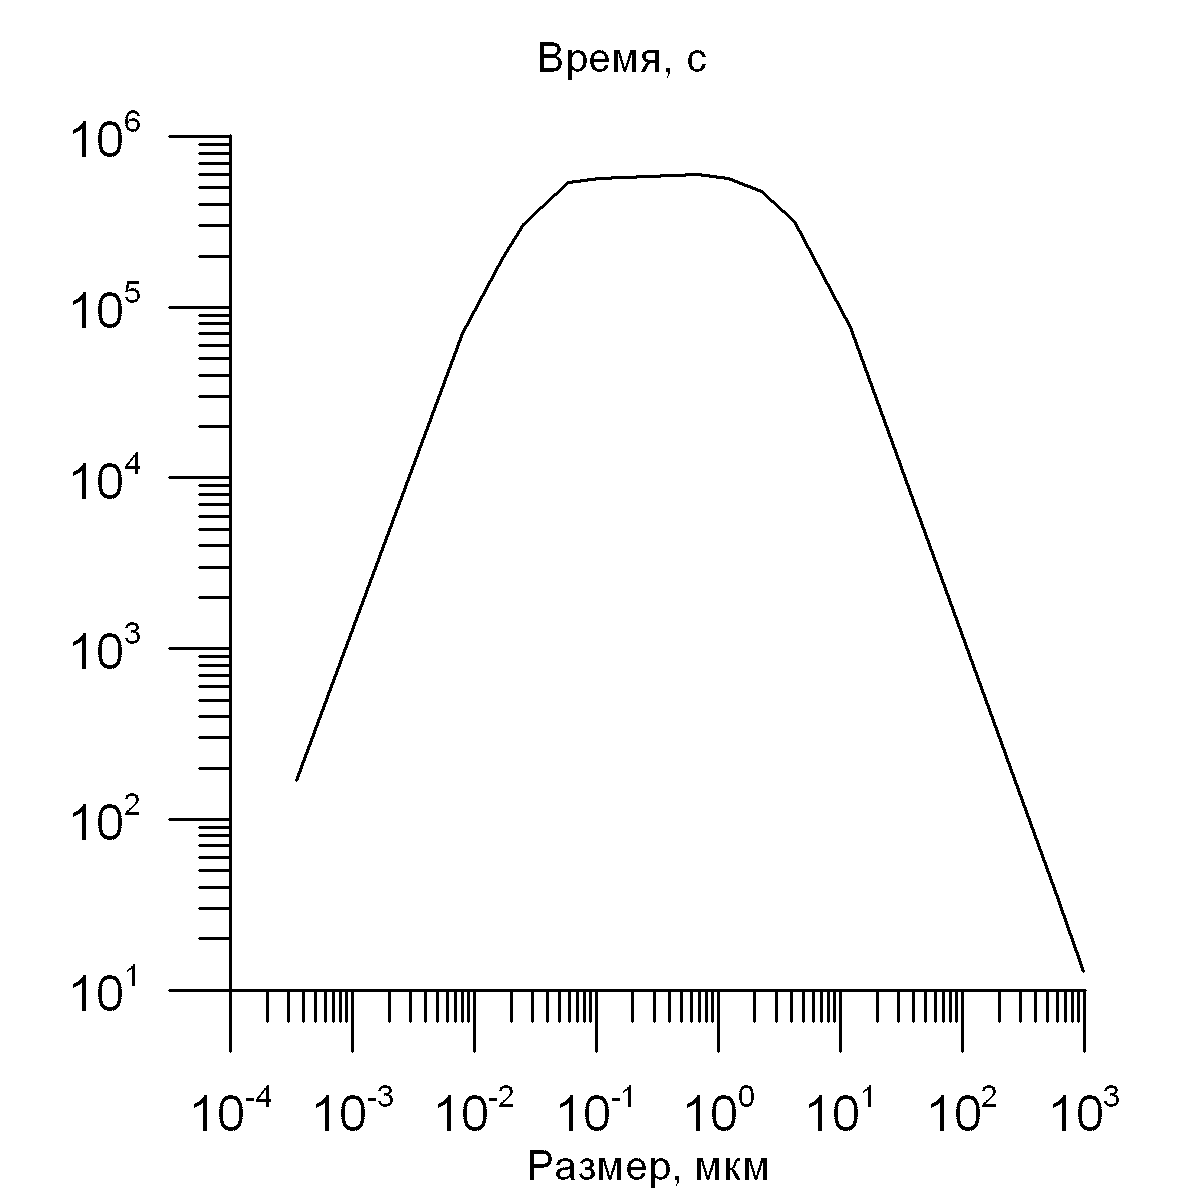
\includegraphics[width=120mm]{pic21}
  \caption{Время жизни пылевых частиц в атмосфере в зависимости от размера частиц на высоте 1.5 км.} 
  \label{img:2lifetime}  
\end{figure}

Действие частиц нано- и макромасштабных размеров на окружающую среду весьма разнообразно за счет влияния на физико-химические свойства атмосферы – начиная от ухудшения видимости из-за рассеяния и поглощения света и заканчивая серьезными климатическими изменениями. Воздействие пыли на атмосферу заметно различается в зависимости от ее химического состава и размера частиц. Поэтому для оценки последствий массовых взрывов на карьерах необходимо знать такие характеристики пыли как химический и гранулометрический состав. 

\section{Эксперимент 9 февраля 2006 года} \label{sect2_3}

9 февраля 2006 г. на Лебединском ГОКе был проведен плановый массовый взрыв общей массой 2 156 т. Было разрушено 15 блоков горной породы. Параметры массового взрыва приведены в табл.~\ref{table:blocks}: номера взрываемых блоков, масса взрывчатых веществ в каждом блоке, число скважин и групп, задержка взрыва соответствующего блока по отношению к моменту начала взрыва блока 31. Блок 31 состоял из известняка, остальные блоки – из железистого кварцита. Расположение блоков представлено на рис.~\ref{img:2blocks}.

\begin{figure} [h] 
  \center
  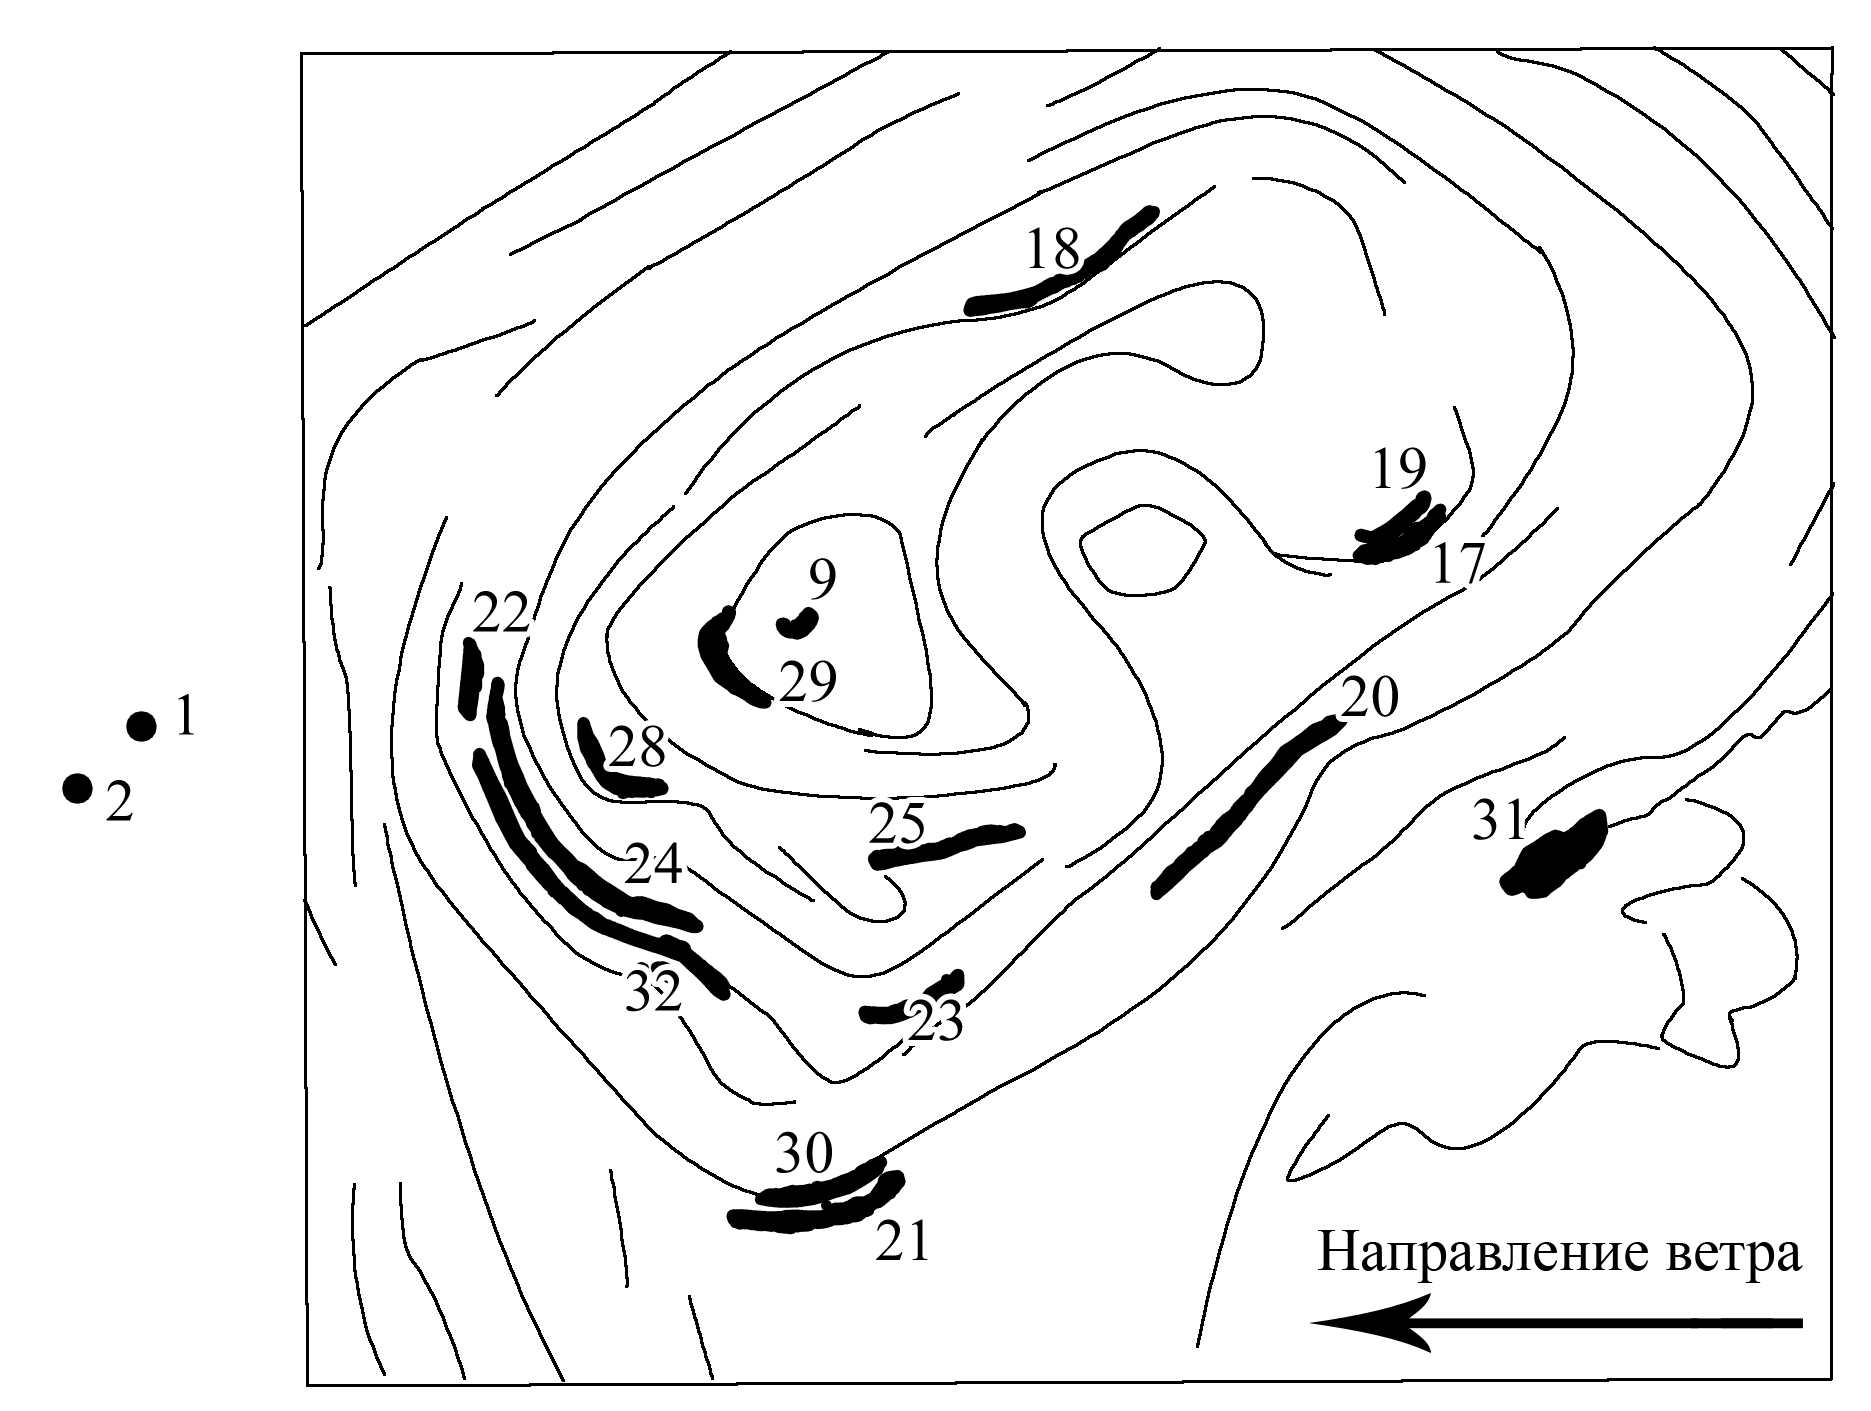
\includegraphics[width=160mm]{pic22}
  \caption{Схема расположения блоков (отмечены жирными линиями) при массовом взрыве 9 февраля 2006 г. на  Лебединском ГОКе. Нумерация блоков соответствует данным табл. \ref{table:blocks}. В точках 1, 2 проводился сбор нано- и микромасштабных частиц.} 
  \label{img:2blocks}  
\end{figure}

\begin{table} [h]
  \centering
  \parbox{16cm}{\caption{Основные параметры массового взрыва}\label{table:blocks}}
  \begin{center}
  \begin{tabular}{| C{1cm} | C{3cm} | C{2cm} | C{1.5cm} | C{2cm} | C{2.5cm} | C{2cm} |}
  \hline
  № блока & Горизонт, м & Масса взрывчатых веществ в блоке, т & Число скважин & Число групп & Средняя масса взрывчатых веществ в группе, т & Задержка взрыва, сек \\
  \hline  
  	31 &   130...125 &  35 &  505 &  44 &  0.795 & 0   \\
	9  &  –180...–195 &  45 &  51 &  19 &  2.37 & 31    \\ 
	29 &  –150...–165 &  130 &  143 &  39 &  3.33 & 31    \\  
	28 &  –75...–90  &  105 &  122 &  32 &  3.28 & 38    \\  
	25 &  –60...–75  &  105 &  118 &  47 &  2.23 & 43    \\  
	24 &  –15...–30  &  340 &  389 &  110 &  3.09 & 67   \\  
	22 &   0...–15  &  410 &  549 &  182 &  2.25 & 67    \\  
	32 &  15...0   &  6.5 &  12 &  6  &  1.08 & 67   \\  
	23 &  –30...–45  &  45 &  60 &  28 &  1.61 & 107   \\  
	30 &  60...45 &   70 &  83 &   34 &  2.06 &  126   \\  
	21 &  75...60  &  185 &  162 &  65 &  2.85 & 126   \\  
	20 &   30...15  &  340 &  260 &  94 &  3.62 & 164   \\  
	19 &  –60...–75  &  55 &  74 &  27 &  2.04 & 195   \\  
	17 &  –45...–60  &  95 &  104 &  33 &  2.88 & 195   \\  
	18 &  –60...–75  &  190 &  206 &  73 &  2.60 & 225   \\
  \hline
  \end{tabular}
  \end{center}
\end{table}


Перед массовым взрывом на разных расстояниях от карьера в направлении ожидаемого ветрового сноса пылевого облака размещались контейнеры для сбора пыли. При данном массовом взрыве контейнеры располагались в двух точках, которые отмечены на рис.~\ref{img:2blocks} черными кружками — 1 и 2. Процесс формирования и распространения облака фиксировался с помощью видеокамер. Сбор выпадающих из пылевого облака твердых частиц осуществлялся в течение всего времени прохождения облака над пунктом наблюдений.

Контейнер для сбора пылевых частиц  представлял собой цилиндрический сосуд диаметром 50 мм и высотой 20 мм, на дне которого размещался фильтр Петрянова (АФА–РСП–10). Чтобы избежать влияния пыления поверхностного слоя грунта в месте проведения измерений, контейнеры располагались на высоте примерно 1 м от земной поверхности.

Было зарегистрировано выпадение твердых частиц из наиболее устойчивого во времени пылевого облака, сформировавшегося в результате взрыва блоков 22 и 24 с общей массой взрывчатых веществ 750 т. Расстояние от центра блоков до точек наблюдения составляло 850 и 970 м.

Усредненный химический состав пыли, выбрасываемой при массовом взрыве, по данным лаборатории Лебединского ГОКа, представлен в табл.~\ref{table:chemistry}.

\begin{table} [h]
  \centering
  \parbox{16cm}{\caption{Химический состав пыли}\label{table:chemistry}}
  \begin{center}
  \begin{tabular}{| C{5cm} | C{3cm} |}
  \hline
  Компоненты & Содержание, \% \\
  \hline  
         $FeO$   &    13.76     \\
         $Fe_{2}O_{3}$   &    24.51     \\
         $SiO_{2}$   &    42.3     \\
         $Al_{2}O_{3}$   &    5.08     \\
         $CaO$   &    1.72     \\
         $MgO$   &    3.27     \\
         $TiO_{2}$   &    0.34     \\
         $P_{2}O_{3}$   &    0.21     \\
         $Na_{2}O$   &    0.33     \\
         $S$   &    0.48     \\

  \hline
  \end{tabular}
  \end{center}
\end{table}

\section{Исследование свойств частиц} \label{sect2_4}

Образец пыли, осажденный на фильтр из пылевого облака, использовался для проведения анализа минералогии и морфологии частиц, а также их гранулометрического состава. Для получения интегрального минерального состава пыли применялся рентгеноструктурный анализ. С помощью дифрактометра "Siemens D5000" ($CuK\alpha$-излучение, длина волны излучения 0.15406 нм) и графитового монохроматора была получена дифрактограмма (фиг.~\ref{img:2difra}) порошкообразного образца с Лебединского ГОКа. Сканы были проведены для углов рассеяния в диапазоне от $2\,^{\circ}$ до $72\,^{\circ}$ ($2\theta$) с шагом $0.03\,^{\circ}(2\theta)$. Дифрактограммы были обработаны с помощью программы "EVA 10.0 (Bruker)".

\begin{figure} [h] 
  \center
  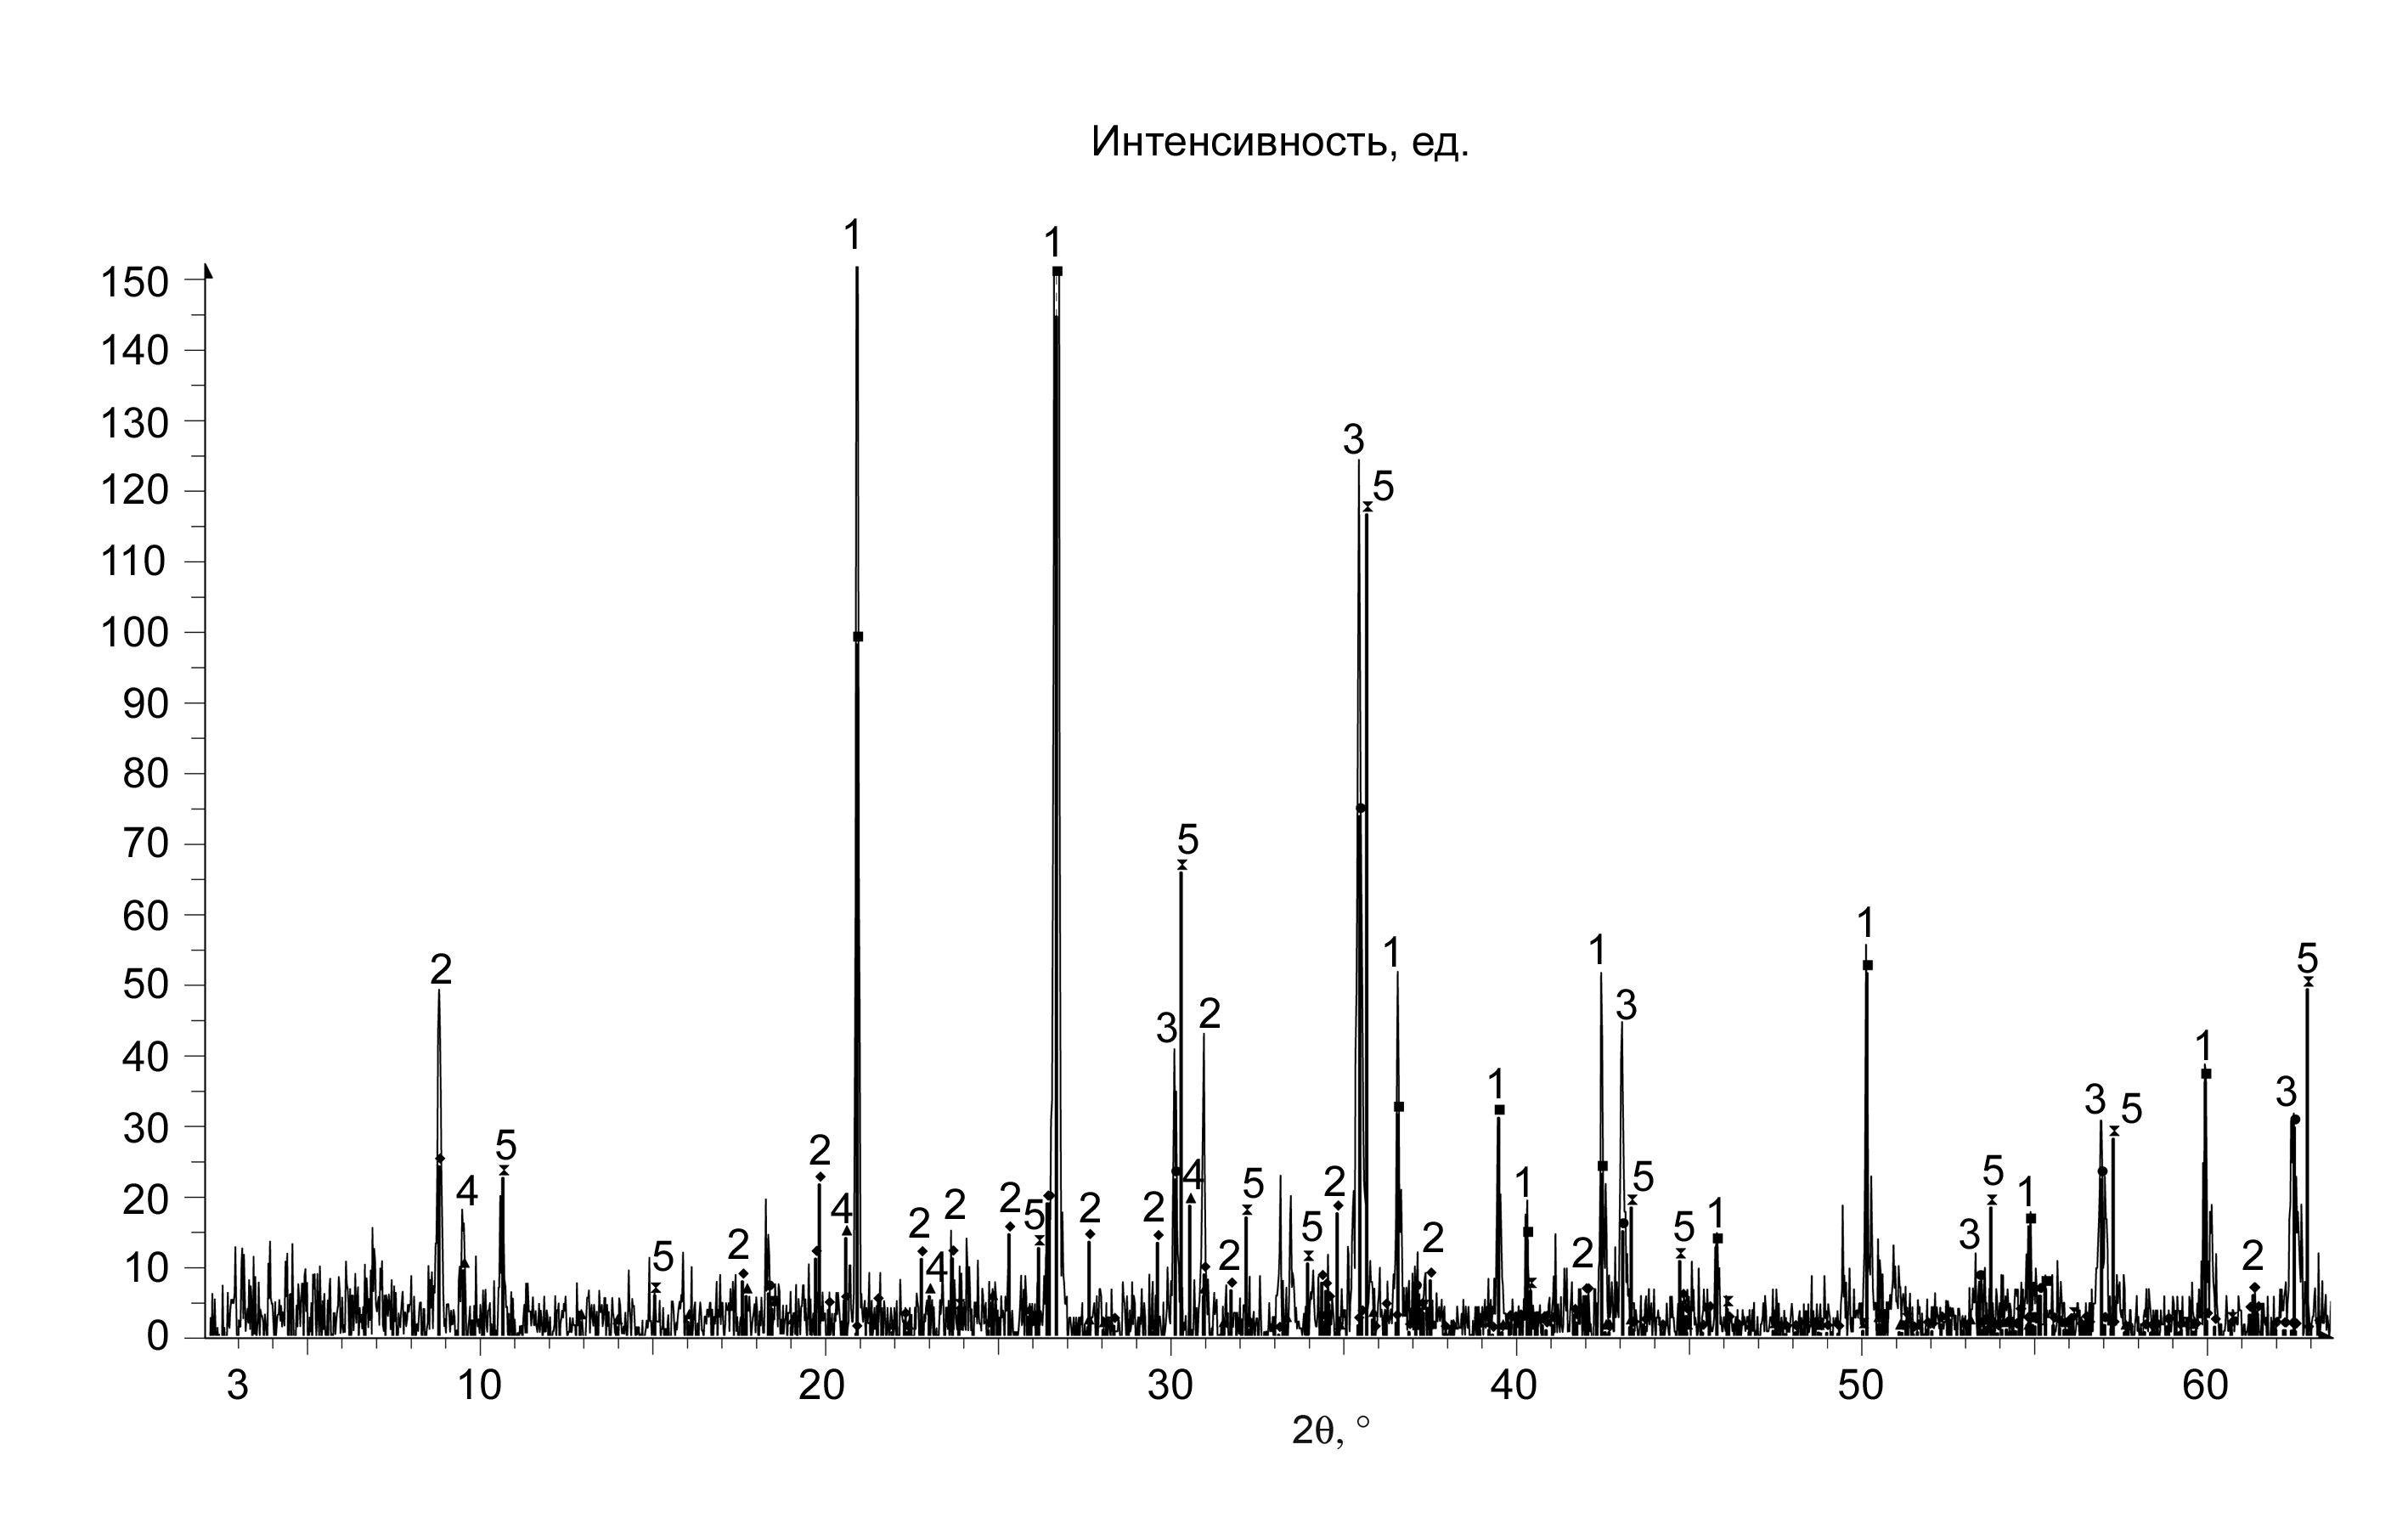
\includegraphics[width=170mm]{pic23}
  \caption{Дифрактограмма рассеяния для порошкообразного образца с Лебединского ГОКа. 1 – кварц; 2 – мусковит; 3 – магнетит; 4 – шабазит; 5 – маггемит.} 
  \label{img:2difra}  
\end{figure}

Основные минеральные фазы, которые были найдены: кварц, магнетит/маггемит, слюда (мусковит/иллит).

В меньшей степени обнаруживаются цеолитоподобные минералы так же, как и Al-, Ca- и Mg- содержащие фазы. Полевые шпаты не выявлены.
Высокое содержание магнитных минералов – магнетита и маггемита – легко демонстрируется прикладыванием постоянного магнита к образцу — ферромагнитные частицы выравниваются вдоль линий магнитного поля. Слабомагнитные частицы собираются на дне стеклянного сосуда.

Для изучения морфологии и поведения частиц образца в зависимости от их минерального состава был использован растровый электронный микроскоп “Philips XL 30 FEG” при ускоряющем напряжении 15 кВ и давлении в вакуумной камере порядка 100 Па. Благодаря режиму низкого вакуума и особой конструкции детектора вторичных электронов в микроскопе для подготовки образца не требуется напылять на него углерод или золото, тогда как в обычных высоковакуумных растровых электронных микроскопах напыление необходимо для того, чтобы избежать накопление заряда. 

Энергодисперсионный рентгеновский анализ проводился на детекторе Sapphire Si (Li) от фирмы "EDAX", охлаждаемом жидким азотом, и выполнялся при напряжении 15 кВ. Время измерения менялось от 2 до 10 мин; для получения элементного состава было выполнено 128 кадров с 5-ти минутной записью для каждого.

Типичная для образца область была диагностирована поэлементно. Железосодержащие частицы имеют лучшую, по сравнению с кремнийсодержащими частицами, электропроводность, поэтому они выделяются более контрастно. Частицы кварца четко обозначаются в кремниевом скане. Частицы, видимые одновременно в Mg-, Al-, Si- и K- сканах, определяются как слюда. В незначительном количестве частиц присутствует кальций. На фиг.~\ref{img:2morfo} представлены вариации морфологии частиц кварца, слюды и магнетита/маггемита. Для всех частиц была отмечена характерная черта – «налипание» мелких частиц на крупные.

\begin{figure} [H] 
  \center
  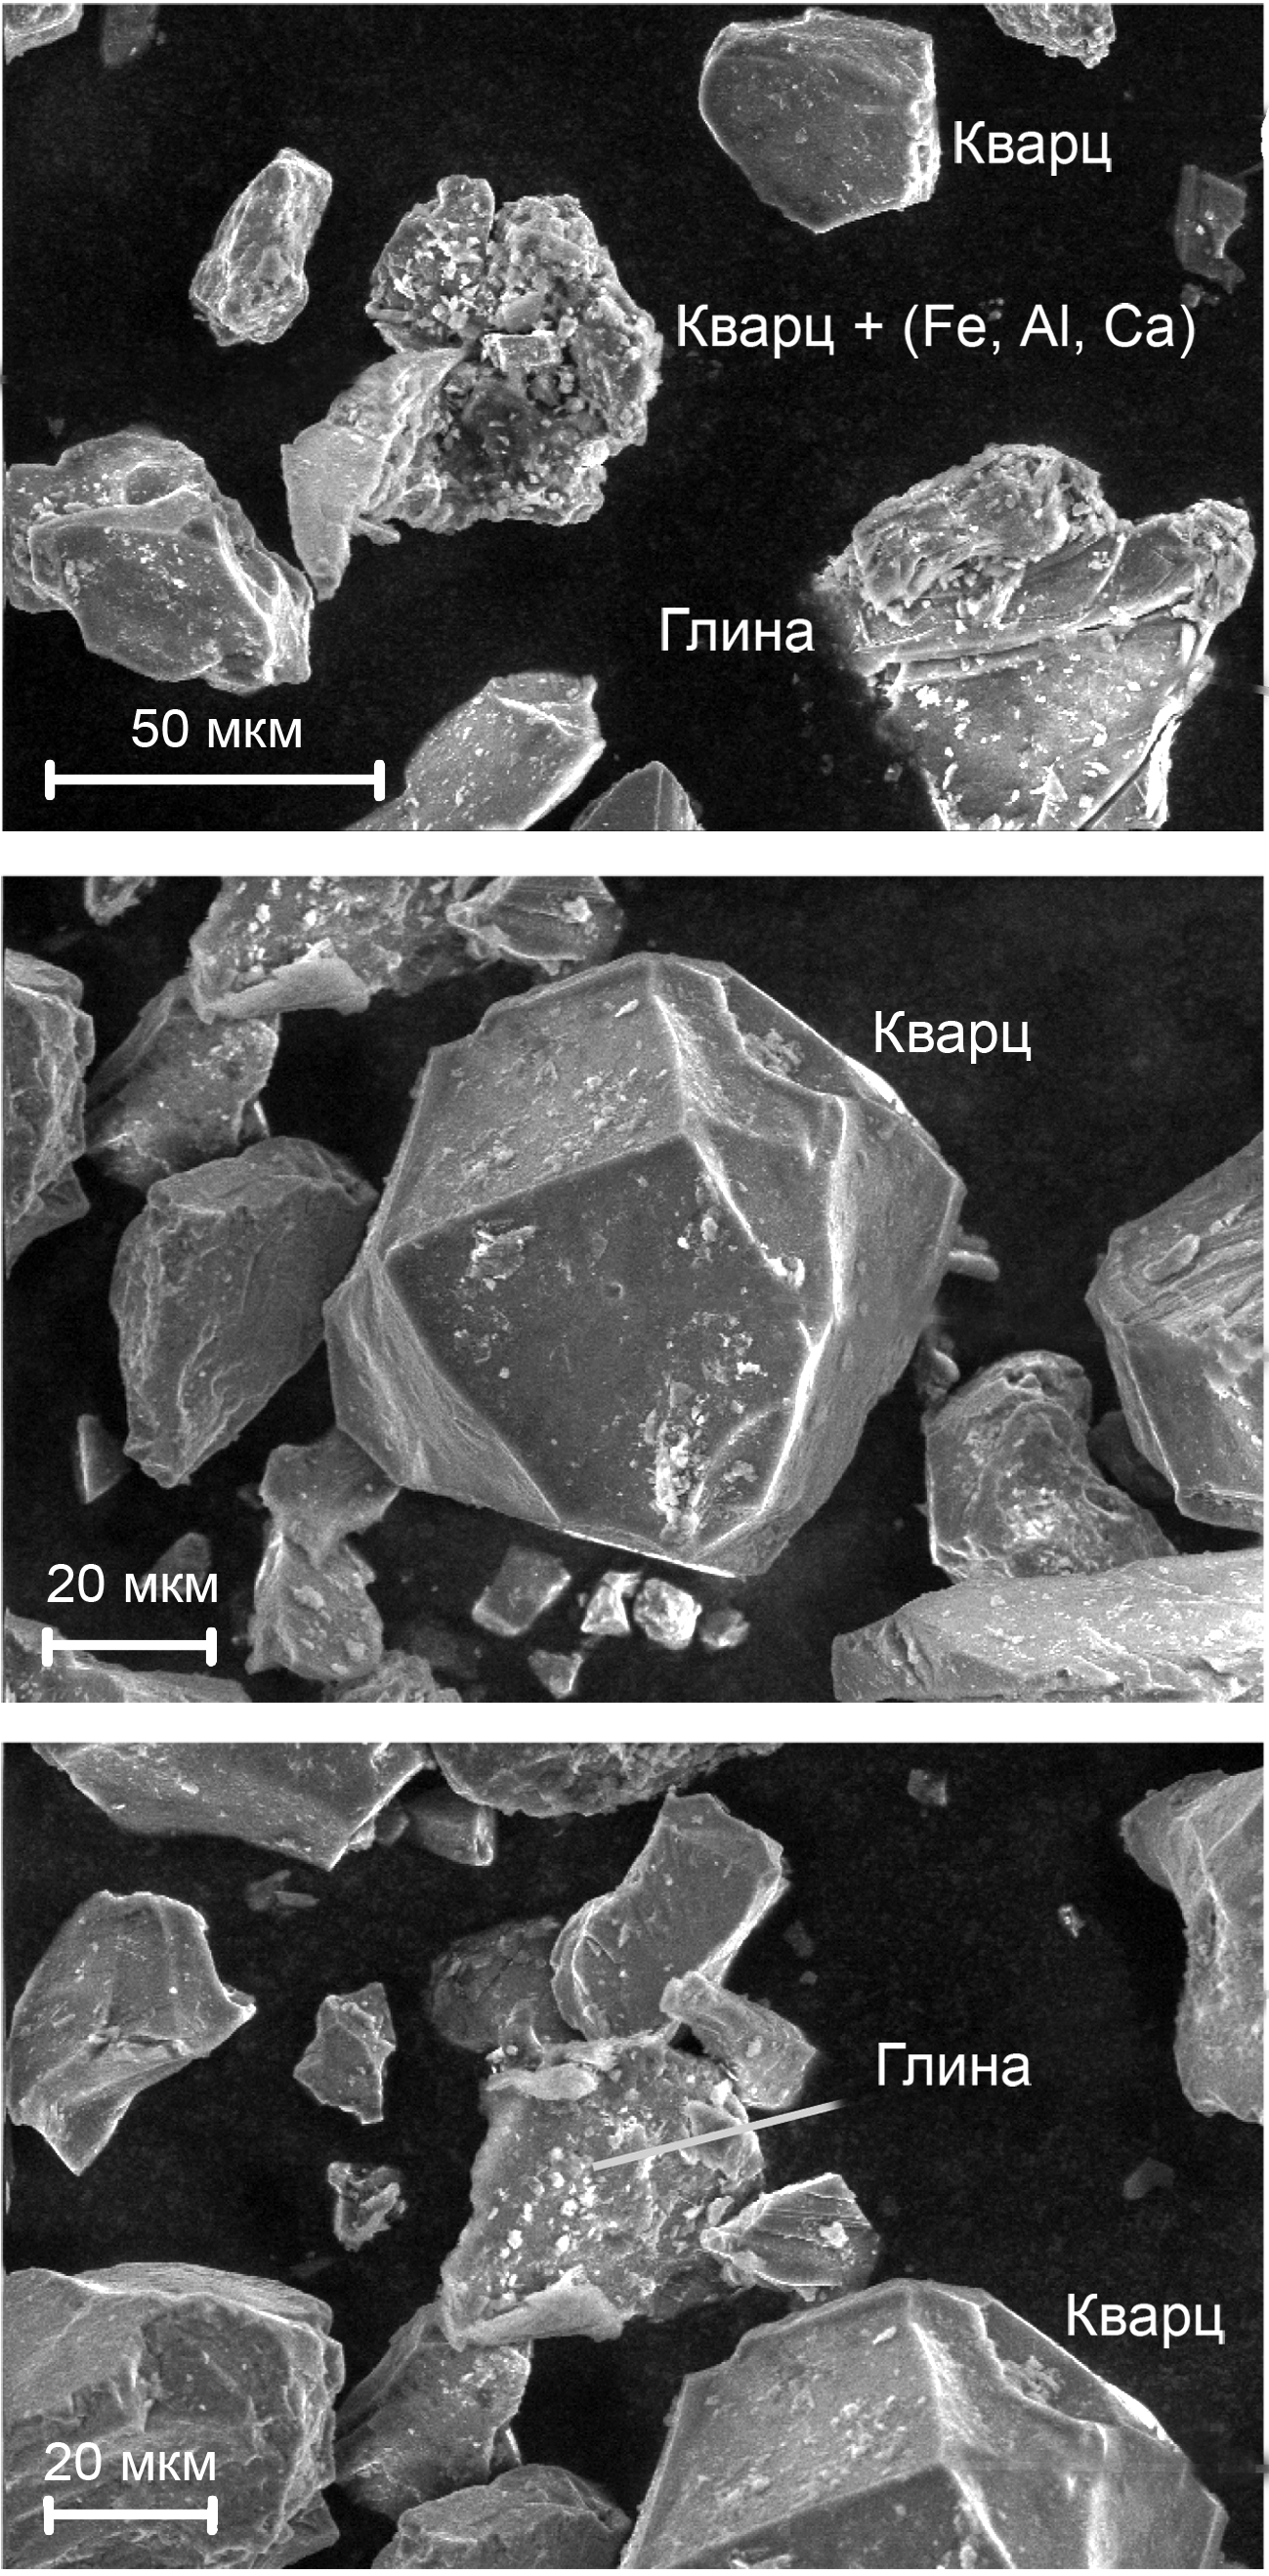
\includegraphics[width=110mm]{pic24}
  \caption{Морфология частиц для кварца и глинистой породы.} 
  \label{img:2morfo}  
\end{figure}

Для определения гранулометрического состава пыли были получены изображения частиц с помощью растрового электронного микроскопа "JEOL 6460 LV" в диапазоне увеличений от 30 до 150 000. Съемка производилась при ускоряющем напряжении 30 кВ и рабочем расстоянии от 8 до 10 мм в режиме высокого вакуума. После общей обработки изображений было получено распределение количества частиц в зависимости от размера от 60 нм (предел разрешения микроскопа) до 200 мкм. 

Для удобства получения информации о размерах частиц и объединения результатов анализа в единую систему было реализовано программное обеспечение \cite{bib10}. Основная задача программы – суммирование информации о количестве и размерах частиц с разных снимков и получение итогового распределения по размерам. Итоговое распределение получается благодаря приведению всех снимков в один масштаб: путем умножения количества частиц на отношение единичной площади к площади снимка. Частицы, налипшие на другие частицы, анализируются отдельно, при этом вместо единичной площади учитывается суммарная площадь свободных частиц.

Результаты подсчета свободных и налипших частиц для образца с Лебединского ГОКа показаны на фиг.~\ref{img:2dispers}. Данные характеризуются тем, что практически все частицы наномасштабного размера находятся на поверхности более крупных и отсутствуют в свободном виде. Этот результат свидетельствует об образовании наномасштабных частиц при взрывах на карьере и об их низкой скорости стока по сравнению с микромасштабными частицами.

\begin{figure} [H] 
  \center
  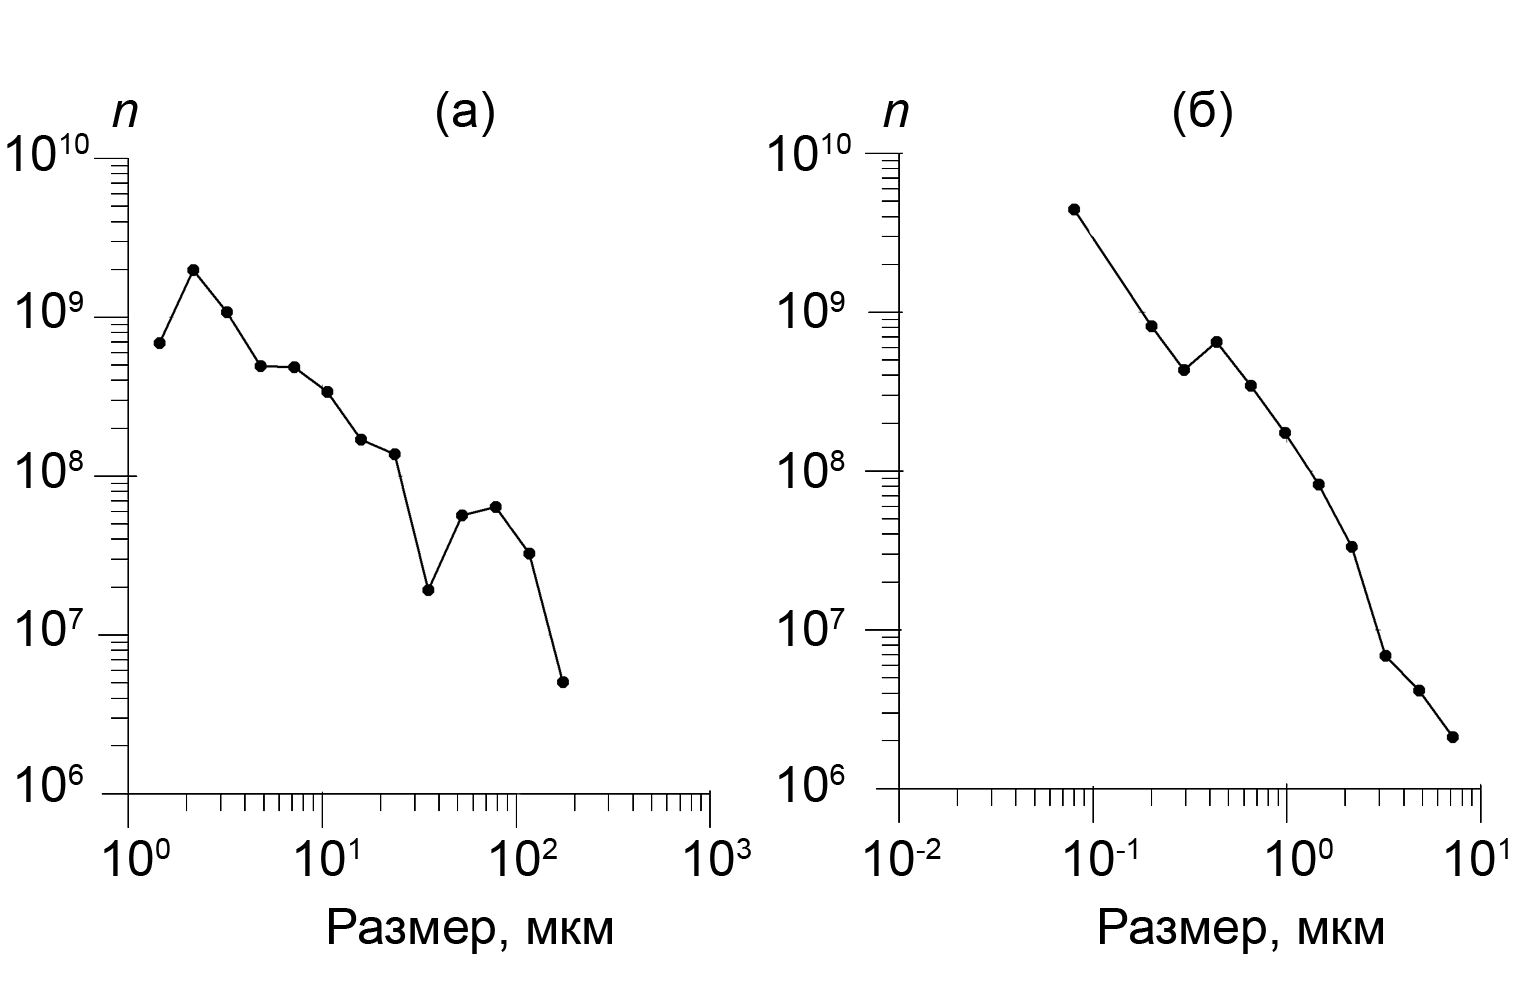
\includegraphics[width=170mm]{pic25}
  \caption{Распределение по размерам частиц, выпавших из пылевого облака после массового взрыва на Лебединском ГОКе 9 февраля 2006 г. Свободные частицы (а) и налипшие на другие частицы (б). $n$ – число частиц. } 
  \label{img:2dispers}  
\end{figure}

Для анализа размерно-массовых соотношений также были построены распределения (фиг. ~\ref{img:2rozinrammler}) в координатах Розина–Раммлера \cite{bib13}. Видно, что обе зависимости хорошо спрямляются в координатах для теоретического распределения Розина–Раммлера, которое характерно для однократного дробления: 
$$
m(x) = m_{0} \exp ⁡\left( - \frac{x}{x_{0}} \right) ^{n},
$$
где $x$ – размер частицы, $m_{0}$ – общая масса вещества, $m(x)$ – общая масса частиц, размер которых больше $x$, а $x_{0}$, $n$ – параметры распределения. 

Количество частиц при разрушении горной массы на Лебединском ГОКе определяется в соответствии с распределением Розина–Раммлера при значении параметров распределения $n$ = 0.8 и $x_{0}$ = 0.6 м \cite{bib11}. При этом в атмосферу выбрасываются частицы пыли с размерами менее 300 мкм. Масса частиц с размерами от 60 нм до 1.5 мкм, которые неэффективно осаждаются, при данных предположениях, составит 0.4 г на 1 кг взрывчатого вещества или 0.8 кг после каждого массового взрыва на Лебединском ГОКе.

\begin{figure} [H] 
  \center
  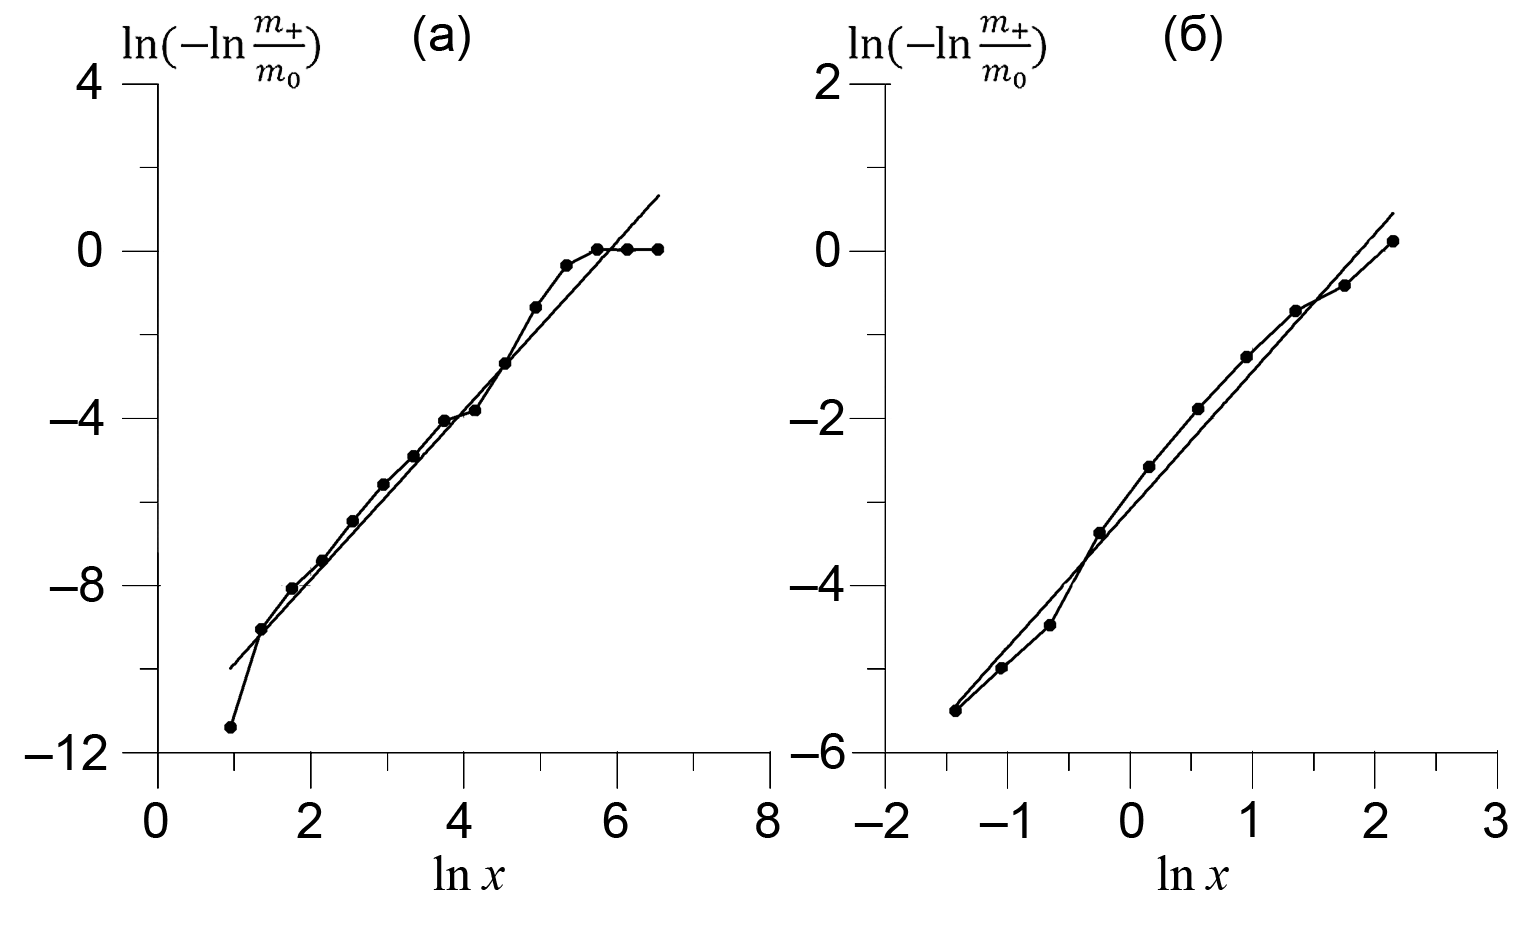
\includegraphics[width=170mm]{pic26}
  \caption{Кривая распределения частиц по размерам в координатах Розина–Раммлера для свободных (а) и налипших (б) частиц.} 
  \label{img:2rozinrammler}  
\end{figure}

\section{Заключение} \label{sect2_5}

Приведены результаты исследований нано- и микромасштабных пылевых частиц, образованных при массовом взрыве на карьере Лебединского ГОКа. В ходе исследований получены данные о морфологии частиц, их магнитных свойствах, минералогическом и гранулометрическом составах. Обнаруженные минералы — кварц, магнетит и слюда. Основная часть пыли состоит из частиц разнообразной морфологии железистого кварцита, в массиве которого и производился взрыв. Существуют гипотезы о том, что железо токсично из-за его способности образовывать сильно окисляющий гидроксил-радикал. В биологических системах гидроксил-радикал может привести, например, к разрыву ДНК \cite{bib17}. Широкий спектр размеров частиц в образце – от 60 нм (предел разрешения микроскопа) до 200 мкм – предполагает разнообразное воздействие их на окружающую среду, так как включает три интервала размеров с качественно разным поведением частиц. Частицы с размерами меньшими 50 нм могут оказаться высоко токсичными \cite{bib06}. Осаждаясь в больших количествах в легких человека, они затормаживают или губят фагоциты, снижая способность организма к выведению посторонних частиц. Также, ввиду малого размера, эти частицы могут пересекать эпителиальный барьер и далее разноситься по всем органам. Частицы с размерами от 100 нм до 2.5 мкм эффективно влияют на рассеяние видимого света, вызывая понижение видимости и нарушая климатический баланс. В ближней окрестности карьера (до 5 км) выпадение частиц наномасштабных размеров, вследствие их низкой скорости стока по сравнению с микромасштабными, осуществляется в основном за счет налипания на поверхность более крупных частиц. При этом основная часть частиц наномасштабных размеров остается в облаке и разносится на большие расстояния от карьера.



\clearpage